\documentclass[10pt, conference, letterpaper]{IEEEtran}
\usepackage{cite}
\usepackage{amsmath,amssymb,amsfonts}
\usepackage{algorithmic}
\usepackage{graphicx}
\usepackage{textcomp}
\usepackage{xcolor}
\usepackage{hyperref}
\usepackage{booktabs}
\usepackage{multirow}
\usepackage{url}
\usepackage{algorithm}

\def\BibTeX{{\rm B\kern-.05em{\sc i\kern-.025em b}\kern-.08em
    T\kern-.1667em\lower.7ex\hbox{E}\kern-.125emX}}

\begin{document}

\title{Double-Blind PQC: A Practical Application-Layer Framework for Integrating NIST Post-Quantum Cryptography in Virtual Private Networks\\
}

\author{\IEEEauthorblockN{Name 1 \\ Name 2}
\IEEEauthorblockA{\textit{School of Computer Science \& Engineering} \\
\textit{Vellore Institute of Technology, Chennai Campus}}
}

\maketitle

\begin{abstract}
The continued advancement of quantum computing poses a serious threat to modern public-key cryptographic systems. Algorithms that depend on integer factorization (RSA) or problems related to elliptic curves and discrete logarithms, like those used in cryptography, will become vulnerable once large-scale, fault-tolerant quantum processors become available. The ``Store Now, Decrypt Later'' (SNDL) attack model, in which adversaries archive encrypted traffic today for future quantum decryption, elevates this from a long-term concern to a present-day cybersecurity imperative.

In this paper, we present \textit{Double-Blind PQC}, an end-to-end software framework that integrates NIST-standardized post-quantum algorithms into a VPN tunneling architecture. Our design pairs ML-KEM-768 (Kyber) for key encapsulation with ML-DSA-65 (Dilithium) for digital signature authentication, and wraps all data traffic in an AES-256-GCM symmetric encryption layer.

A key contribution of this work is a deterministic Application-Layer Fragmentation Wrapper that addresses the practical challenge of transmitting multi-kilobyte post-quantum keys and signatures over UDP, a protocol where the payloads often go beyond the standard Maximum Transmission Unit (MTU). We benchmark our system against widely deployed classical primitives - X25519, SECP256R1, RSA-3072, and Ed25519 - and demonstrate that ML-KEM-768 achieves key generation latencies that consistently outperform even elliptic curve methods, confirming the practical viability of deploying PQC in real-world VPN environments.
\end{abstract}

\begin{IEEEkeywords}
Post-Quantum Cryptography, CRYSTALS-Kyber, CRYSTALS-Dilithium, SPHINCS+, Falcon, VPN, WireGuard, Network Security, Key Encapsulation Mechanism, Latency Evaluation, MTU Fragmentation
\end{IEEEkeywords}

\section{Introduction}

\subsection{The Quantum Threat Horizon}
The security of modern internet communications depends almost entirely on public-key cryptography. Protocols such as IPsec, OpenVPN, TLS~1.3, and WireGuard negotiate session keys using Elliptic Curve Cryptography (ECC), most commonly via the X25519 curve \cite{hulsing2017pqwireguard}. These schemes derive their security from the computational difficulty of solving discrete logarithm or integer factorization problems - tasks that remain intractable for classical computers.

Shor's algorithm, introduced in 1994, changes this calculus entirely. A sufficiently powerful quantum computer running Shor's algorithm can solve both integer factorization and elliptic curve discrete logarithms in polynomial time, rendering RSA, ECDHE, and related schemes fundamentally broken. Additionally, Grover's algorithm provides a quadratic speedup for a brute-force search, this would essentially cut the security level in half, making it a whole lot easier to crack symmetric ciphers like AES. An AES-128 key, for example, would only provide 64 bits of security if a quantum computer were to attack it, necessitating a transition to AES-256 as the minimum standard \cite{shim2025qtrustnet}.

What makes the quantum threat urgent rather than merely theoretical is the SNDL attack model. Nation-state adversaries and other well-resourced actors are already intercepting and archiving vast volumes of encrypted traffic. When cryptographically relevant quantum computers (CRQCs) eventually come online, this archived data can be retroactively decrypted. For sensitive communications with long confidentiality requirements - government, military, financial, or medical records - the window for action is now, not when quantum computers arrive.

\subsection{NIST PQC Standardization and Strategic Context}
In response to the quantum threat, NIST launched a multi-year standardization effort to identify cryptographic algorithms resistant to both classical and quantum attacks. Candidate algorithms, spanning structured lattices, code-based systems, isogeny-based schemes, and multivariate polynomials, were evaluated across multiple rounds of public cryptanalysis. Selection criteria included computational efficiency, key and signature sizes, and provable security guarantees.

The process concluded with the selection of ML-KEM (derived from CRYSTALS-Kyber) for key encapsulation and ML-DSA (derived from CRYSTALS-Dilithium) for digital signatures as the primary standards. Both are built on the Module Learning With Errors (MLWE) problem over polynomial lattices, a mathematical foundation widely believed to resist quantum attacks.

NIST also standardized two additional signature schemes: Falcon, a lattice-based scheme that produces notably compact signatures and is well-suited for bandwidth-constrained environments, and SPHINCS+, a stateless hash-based scheme whose security relies solely on the properties of hash functions rather than lattice assumptions. SPHINCS+ offers a valuable fallback in the event that lattice-based schemes are compromised by future cryptanalytic advances, though its larger signature sizes and slower performance limit its suitability for latency-sensitive network protocols. In practice, ML-DSA and Falcon remain the primary candidates for VPN authentication.

\subsection{Architectural Transport Integration Hurdles}
While the mathematical security of MLWE-based algorithms is well-established, integrating them into existing network infrastructure presents significant engineering challenges. Current VPN implementations are optimized for the compact key sizes of classical ECC - an X25519 public key is just 32 bytes. By contrast, an ML-KEM-768 public key requires 1,184 bytes, and an ML-DSA-65 signature exceeds 3,000 bytes.

These enlarged payloads create problems at the transport layer. When sent over UDP - the preferred protocol for high-performance VPNs - payloads exceeding the standard Ethernet MTU of 1,500 bytes trigger IP-level fragmentation. Under UDP, if any single fragment is lost in transit, the entire datagram is silently discarded, with no retransmission mechanism. In reality, this means that simply integrating Post-Quantum Cryptography, or PQC, isn't a reliable solution and can prevent tunnel establishment entirely \cite{shim2025qtrustnet}.

\section{Background and Literature Review}

\subsection{Post-Quantum WireGuard}
H\"ulsing et al. \cite{hulsing2017pqwireguard} introduced PQ-WireGuard, one of the earliest efforts to retrofit the WireGuard VPN protocol with post-quantum security. Their approach replaced WireGuard's standard Diffie-Hellman key exchange, which relies on interactive curve operations, with a unidirectional KEM-based handshake. Using formal verification tools, they demonstrated that the resulting protocol is cryptographically sound.

However, their evaluation also revealed a significant performance penalty during the handshake phase. The large key and ciphertext sizes inherent to post-quantum KEMs introduce measurable latency overhead compared to the original 32-byte X25519 handshake. This work highlighted the tension between quantum resistance and transport efficiency that motivates our own research.

\subsection{qTrustNet and Hardware-Bound PQC Interfaces}
Shim et al. \cite{shim2025qtrustnet} took a different approach with qTrustNet, a VPN architecture that combines NIST PQC algorithms with hardware-level security primitives. Their design integrates post-quantum key exchange directly into WireGuard transport endpoints while securing local key storage using Physically Unclonable Functions (PUFs), which bind cryptographic material to the physical characteristics of individual hardware devices.

Their experimental results demonstrated low-latency operation with sustained throughput approaching 8.5~Gbps on 10GbE network interfaces. The architecture provides strong security guarantees, but its dependence on specific hardware components (PUF devices, kernel-level WireGuard modifications) limits portability across heterogeneous environments.

\subsection{Identifying the Application-Layer Gap}
Both PQ-WireGuard and qTrustNet operate at or near the kernel level, requiring either modifications to WireGuard's internal protocol state machine or dedicated hardware security modules. While effective, these approaches are difficult to deploy across diverse operating systems and network configurations.

The Double-Blind PQC framework addresses this gap by operating entirely at the application layer. Rather than modifying kernel modules or requiring specialized hardware, our system manages PQC key exchange, signature verification, and MTU-compliant fragmentation within a standard userspace process. This design choice sacrifices some raw throughput compared to kernel-integrated solutions, but gains broad compatibility: the same codebase runs on any platform with a Python interpreter and access to the underlying PQC libraries, without requiring root access, kernel patches, or vendor-specific hardware.

\section{Threat Model and Assumptions}
We define the following threat model, which represents a worst-case scenario for public internet communication under quantum-era conditions:

\begin{itemize}
    \item \textbf{Dolev-Yao Network Adversary}: The adversary has complete control over the network channel between the Initiator and Responder nodes. They can intercept, read, modify, delay, reorder, replay, or drop any UDP packet in transit.
    \item \textbf{Quantum Computing Capability}: The adversary either currently possesses or will eventually obtain access to a CRQC capable of running Shor's and Grover's algorithms. All recorded traffic is assumed to be vulnerable to future decryption.
    \item \textbf{Endpoint Integrity}: We assume that the VPN client endpoints themselves are uncompromised - free from malware, side-channel vulnerabilities, or physical tampering. The endpoints are treated as trusted platforms.
\end{itemize}

Under this threat model, the protocol must provide two core guarantees: (1)~mutual authentication, preventing man-in-the-middle attacks even against an active quantum-capable adversary, and (2)~forward secrecy, ensuring that compromise of long-term keys does not reveal past session keys. Both guarantees rest on the assumed hardness of the MLWE problem against quantum algorithms.

\section{Cryptographic Foundation and Architecture}

The Double-Blind PQC framework combines three cryptographic primitives into a single protocol flow: a lattice-based KEM for key agreement, a lattice-based signature scheme for authentication, and a symmetric cipher for bulk data encryption. This section describes each component and the protocol that ties them together.

\subsection{Cryptographic Primitives}

\textbf{1) ML-KEM-768 (CRYSTALS-Kyber):} ML-KEM-768 serves as the key encapsulation mechanism. Unlike traditional Diffie-Hellman, which requires an interactive exchange of curve points, KEM-based protocols follow a three-step process:
\begin{enumerate}
    \item \textit{Key Generation}: The Initiator generates a Kyber keypair and publishes the 1,184-byte public key $PK_{KEM}$.
    \item \textit{Encapsulation}: The Responder uses $PK_{KEM}$ to encapsulate a random 32-byte shared secret $SS$, producing a 1,088-byte ciphertext $CT$.
    \item \textit{Decapsulation}: The Initiator recovers $SS$ from $CT$ using the corresponding private key $SK_{KEM}$.
\end{enumerate}
ML-KEM-768 targets a security level roughly equivalent to AES-192, and its performance characteristics - particularly key generation speed - compare favorably to classical alternatives, as we demonstrate in Section~VI.

\textbf{2) ML-DSA-65 (CRYSTALS-Dilithium):} All handshake messages are authenticated using ML-DSA-65 (Dilithium-3) digital signatures. Dilithium uses a ``Fiat-Shamir with Aborts'' construction that prevents information leakage through signature values - a concern with earlier lattice-based signature designs.

The downside is that it's big: Dilithium public keys are 1,952 bytes in size, and signatures are 3,293 bytes. These are an order of magnitude larger than Ed25519's 32-byte keys and 64-byte signatures, and they represent the primary driver of the MTU challenges discussed in Section~V.

\subsection{Handshake Protocol}

The Double-Blind handshake follows a 1-RTT (single round-trip) model. We assume that both the Initiator ($I$) and Responder ($R$) possess pre-provisioned long-term ML-DSA identity keypairs: ($PK_{sig\_I}$, $SK_{sig\_I}$) and ($PK_{sig\_R}$, $SK_{sig\_R}$), respectively.

\begin{figure}[!t]
\centering
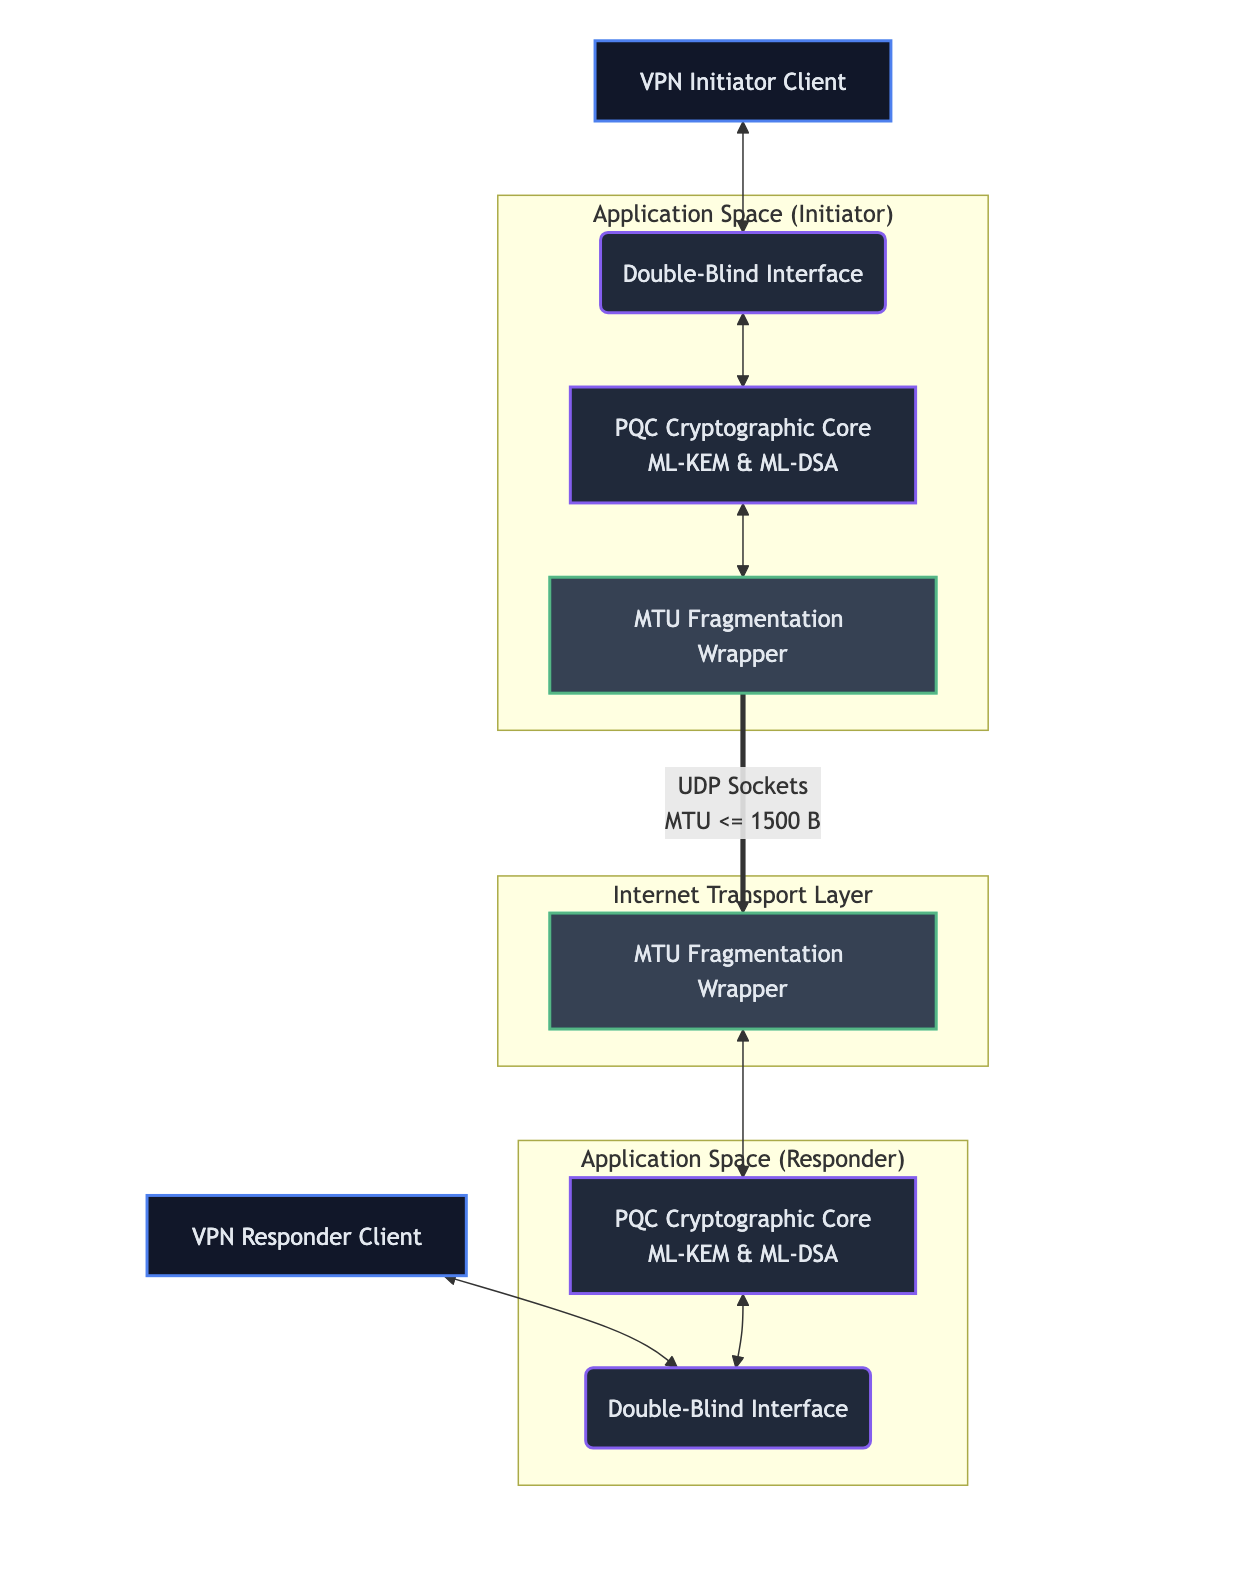
\includegraphics[width=\linewidth]{image.png}
\caption{System architecture showing the separation between application-layer cryptographic operations and kernel-level IP transport.}
\label{fig:architecture}
\end{figure}

\textbf{Step 1: Initiation.} $I$ generates an ephemeral ML-KEM-768 keypair ($PK_{kem\_I}$, $SK_{kem\_I}$) and a random 32-byte nonce $Nonce_{I}$. It signs the concatenation $PK_{kem\_I} \| Nonce_{I}$ using $SK_{sig\_I}$, then transmits the public key, nonce, and signature to $R$. Because the combined payload exceeds the MTU, the fragmentation wrapper (Section~V) splits it into MTU-compliant UDP packets before transmission.

\textbf{Step 2: Validation and Encapsulation.} $R$ reassembles the incoming fragments and verifies the Dilithium signature using $PK_{sig\_I}$. If verification fails, $R$ immediately terminates the connection. Otherwise, $R$ runs KEM encapsulation against $PK_{kem\_I}$ to produce the shared secret $SS$ and ciphertext $CT$. It then signs the combination of $CT$ and $Nonce_{R}$ using $SK_{sig\_R}$ and sends the response back to $I$ via the same fragmentation mechanism.

\textbf{Step 3: Decapsulation.} $I$ reassembles the response, verifies $R$'s signature using $PK_{sig\_R}$, and decapsulates $CT$ with $SK_{kem\_I}$ to recover $SS$. At this point, both parties hold the same 32-byte shared secret and the expensive asymmetric operations are complete.

\begin{algorithm}[H]
\caption{Double-Blind Handshake \& Encapsulation}\label{alg:handshake}
\begin{algorithmic}[1]
\renewcommand{\algorithmicrequire}{\textbf{Input:}}
\renewcommand{\algorithmicensure}{\textbf{Output:}}
\REQUIRE Initiator ID Key $SK_{I}$, Responder ID Key $PK_{R}$
\ENSURE Local Symmetric Session Array Key $SS_{tunnel}$
\STATE \text{Initialize AES-GCM Transport Pipeline}
\STATE $PK_{KEM}, SK_{KEM} \leftarrow ML\_KEM.GenerateKeyPair()$
\STATE $Nonce_I \leftarrow RandomSecureBitGenerator(32)$
\STATE $Payload_{init} \leftarrow (PK_{KEM} || Nonce_I)$
\STATE $Signature_{init} \leftarrow ML\_DSA.Sign(SK_{I}, Payload_{init})$
\STATE $TransmitArray(Payload_{init} || Signature_{init})$
\WHILE{System Wait For Responder Feedback}
    \STATE $Payload_{resp}, Signature_{resp} \leftarrow ReceiveArray()$
    \IF{$!ML\_DSA.Verify(PK_{R}, Payload_{resp}, Signature_{resp})$}
        \STATE \textbf{return} $CONNECTION\_REJECTED\_FATAL$
    \ENDIF
    \STATE $CT_{KEM}, Nonce_R \leftarrow ParseObject(Payload_{resp})$
    \STATE $SS_{tunnel} \leftarrow ML\_KEM.Decapsulate(SK_{KEM}, CT_{KEM})$
    \STATE \textbf{break}
\ENDWHILE
\STATE \textbf{return} $SS_{tunnel}$
\end{algorithmic}
\end{algorithm}

\begin{figure}[!t]
\centering
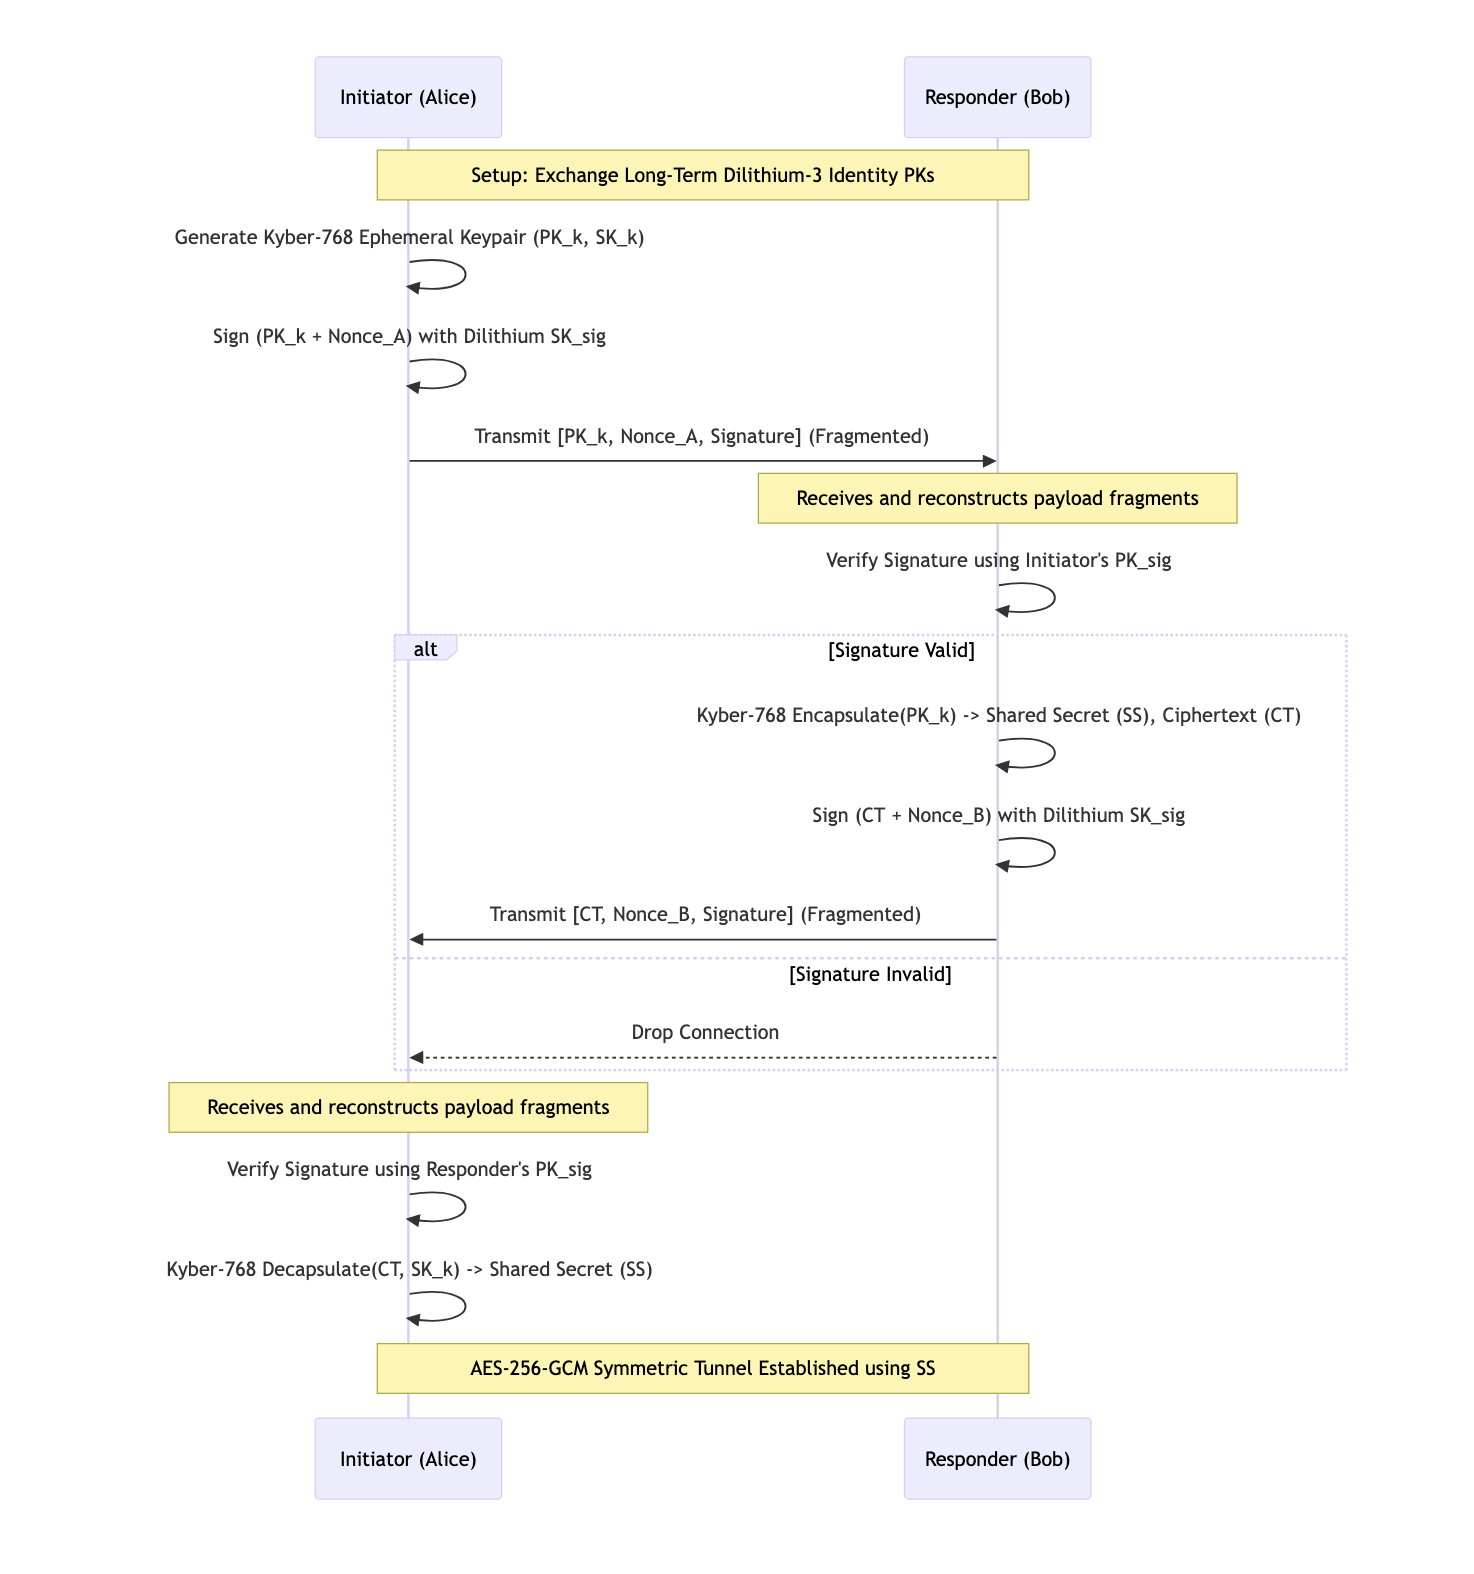
\includegraphics[width=\linewidth]{image2.png}
\caption{Sequence diagram of the Double-Blind PQC handshake protocol.}
\label{fig:sequence}
\end{figure}

\subsection{Symmetric Tunnel Establishment}
Once the handshake completes and both nodes share $SS$, the asymmetric operations are finished. The raw 32-byte secret is expanded through a Key Derivation Function (KDF) based on BLAKE2s to produce a 256-bit symmetric key. This key initializes an \textbf{AES-256-GCM} (Galois/Counter Mode) tunnel for all subsequent data traffic. AES-256 retains 128 bits of security even against Grover's algorithm, which is generally considered sufficient for the foreseeable future \cite{nist2022pqc}.


\section{Network Engineering: Application-Layer Fragmentation}
The large key and signature sizes of post-quantum algorithms create a practical transport problem that must be solved before any PQC VPN can function reliably. This section describes the problem and our solution.

\subsection{The MTU Problem}
Standard Ethernet imposes a Maximum Transmission Unit of 1,500 bytes per frame. After accounting for IP and UDP headers (typically 28 bytes combined), the usable payload per datagram is approximately 1,472 bytes. A single Double-Blind handshake message - containing a Kyber public key, a Dilithium signature, and a one-time nonce - comes out to roughly 4,500 bytes, which is way more than what can fit in a single UDP datagram.

If this oversized payload is handed directly to the OS kernel, the kernel will perform IP-level fragmentation, splitting the datagram into multiple IP fragments. Under UDP, this is unreliable: the loss of any single fragment causes the entire message to be basically lost, and there's no backup plan for retransmission. On congested or lossy networks, this makes handshake completion unpredictable and can prevent tunnel establishment.

\subsection{Deterministic Application-Layer Fragmentation}
To avoid OS-level fragmentation entirely, we implemented a \textbf{Fragmentation Wrapper} at the application layer. Before any data is written to the UDP socket, the wrapper divides it into smaller parts, no more than \texttt{CHUNK\_SIZE} bytes each (set to 1,000 bytes by default, providing margin below the MTU).

Each piece of data starts with a small 6-byte header:
\begin{itemize}
    \item \texttt{Message\_ID} (2 bytes): It's like a special code, a random 16-bit identifier that helps link all fragments of the same original message.
    \item \texttt{Fragment\_Index} (2 bytes): The sequential position of this fragment (0 through $N{-}1$).
    \item \texttt{Total\_Fragments} (2 bytes): The total number of fragments in the message ($N$).
\end{itemize}

Algorithm~\ref{alg:frag} details the fragmentation procedure.

\begin{algorithm}[H]
\caption{Deterministic MTU Payload Extractor}\label{alg:frag}
\begin{algorithmic}[1]
\REQUIRE Encrypted Monolithic Payload $P_{enc}$, Defined $MTU_{limit}$
\ENSURE Sequential List of Compliant UDP Packets $U$
\STATE $L \leftarrow ByteLength(P_{enc})$
\IF{$L \leq MTU_{limit}$}
    \STATE $Header \leftarrow (RandomUInt16() || 0 || 1)$
    \STATE $Transmit(Header || P_{enc})$
    \STATE \textbf{return} 1
\ENDIF
\STATE $N \leftarrow \lceil L / MTU_{limit} \rceil$
\STATE $SessionID \leftarrow RandomUInt16()$
\STATE $U \leftarrow []$
\FOR{$i = 0$ to $N - 1$}
    \STATE $StartBoundary \leftarrow i \times MTU_{limit}$
    \STATE $EndBoundary \leftarrow Minimum((i + 1) \times MTU_{limit}, L)$
    \STATE $ChunkData \leftarrow P_{enc}[StartBoundary : EndBoundary]$
    \STATE $Header \leftarrow (SessionID || i || N)$
    \STATE $U[i] \leftarrow (Header || ChunkData)$
    \STATE $Socket.SendTo(U[i])$
\ENDFOR
\STATE \textbf{return} $N$
\end{algorithmic}
\end{algorithm}

\begin{figure}[!t]
\centering
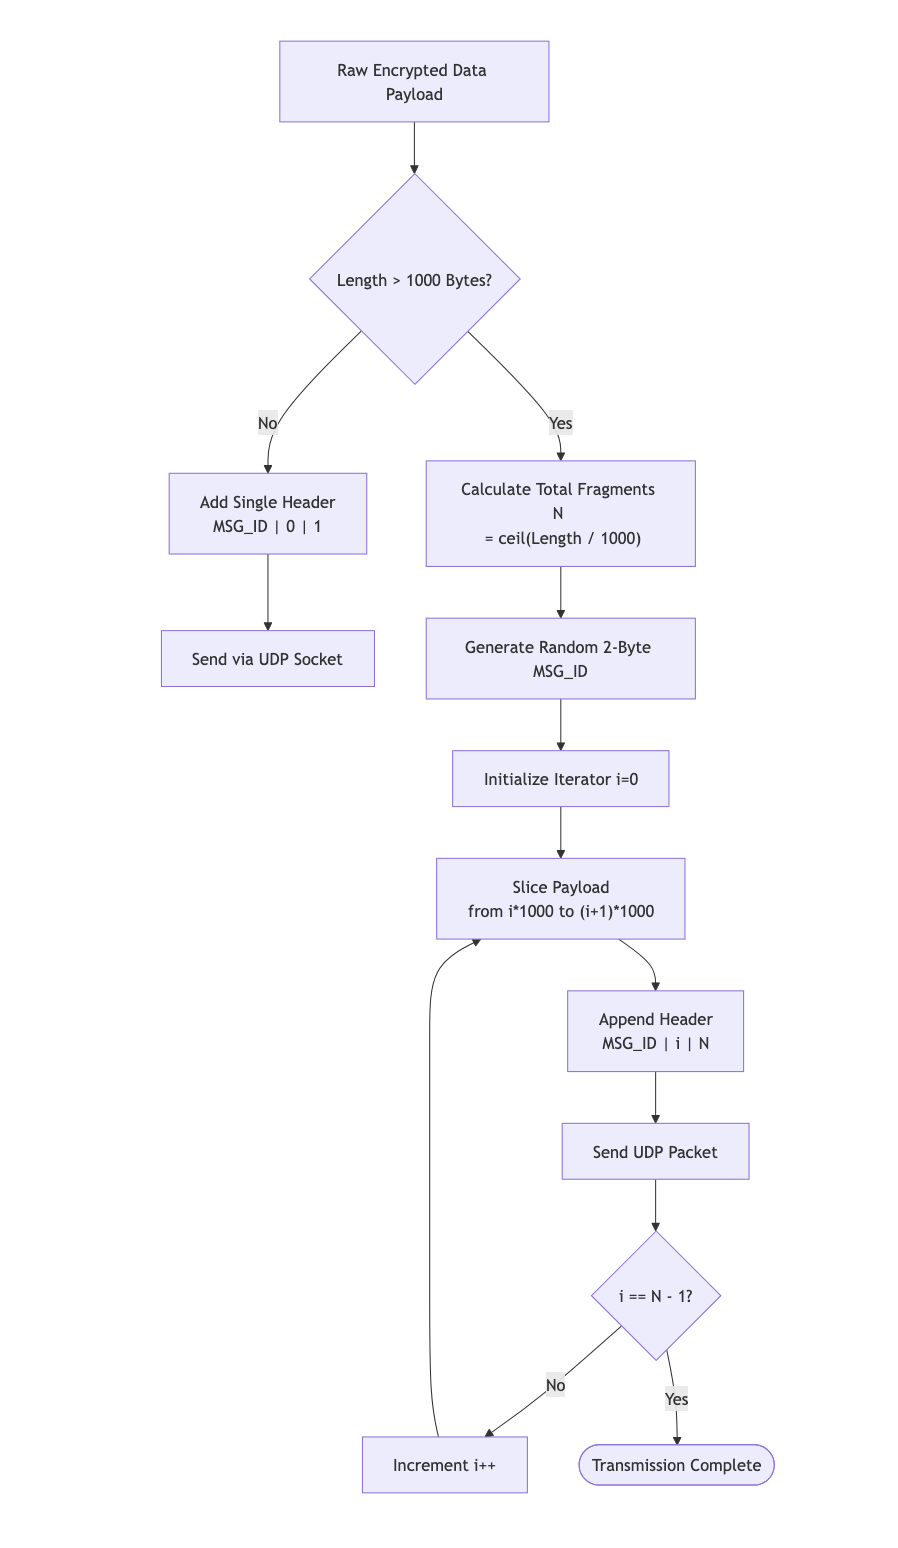
\includegraphics[width=\linewidth]{image3.png}
\caption{Flowchart of the application-layer fragmentation logic.}
\label{fig:fragmentation}
\end{figure}

\subsection{Reassembly and Timeout Handling}
On the receiving side, incoming fragments are buffered in a dictionary keyed by \texttt{Message\_ID}. As fragments arrive - potentially out of order, since UDP provides no ordering guarantees - each is placed into the correct position based on its \texttt{Fragment\_Index}. Once all $N$ fragments for a given \texttt{Message\_ID} have been received, the buffer is simplified into a more manageable format and the original information is sent to the cryptographic layer for processing.

To prevent memory exhaustion from incomplete or malicious fragment streams, the reassembly engine enforces a configurable timeout. If all fragments for a given message are not received within the time limit, only the partial information gets through and is discarded, and the handshake layer may request retransmission. This provides basic resilience against both network instability and denial-of-service attacks targeting the fragment buffer.


\section{Experimental Setup and Performance Analysis}
To evaluate the computational overhead introduced by the Double-Blind PQC framework, we conducted a benchmarking study comparing our post-quantum primitives against widely deployed classical algorithms. The goal was to quantify the real-world performance trade-offs of adopting PQC in a VPN context.

\subsection{Methodology}
The benchmarking suite was integrated into the application's Python backend and executed locally to isolate cryptographic computation times from network latency. We used Python's \texttt{time.perf\_counter()} for high-resolution timing. We ran the algorithm 25 times and the results are based on $N = 25$ iterations, reporting arithmetic means. This iteration count is sufficient to smooth out OS scheduling jitter while keeping benchmark runtime manageable.

The following classical algorithms were selected as baselines for comparison:
\begin{itemize}
    \item \textbf{X25519 (ECDH)}: The elliptic curve used by WireGuard; represents the current state of the art in VPN key exchange.
    \item \textbf{SECP256R1 (P-256)}: The NIST standard elliptic curve, widely used in TLS and corporate VPN products.
    \item \textbf{Ed25519}: A high-performance Edwards curve signature scheme commonly used for SSH and code signing.
    \item \textbf{RSA-3072 / RSA-PSS}: Traditional integer-factorization-based cryptography, included as a legacy baseline.
\end{itemize}

\subsection{Key Encapsulation Results}
Table~\ref{tab:kem} presents the key generation and encapsulation/exchange latencies for each KEM or key-agreement algorithm.

\begin{table}[hbt!]
\centering
\caption{KEM / Key Exchange Performance (mean of 25 iterations)}
\label{tab:kem}
\resizebox{\columnwidth}{!}{
\begin{tabular}{l c c c c}
\toprule
\textbf{Algorithm} & \textbf{KeyGen (ms)} & \textbf{Exch/Encap (ms)} & \textbf{Pub Key (B)} \\
\midrule
ML-KEM/Kyber-768 & 0.063 & 0.081 & 1184 \\
X25519 (ECDH) & 0.174 & 0.235 & 32 \\
P-256 (SECP256R1) & 0.355 & 0.442 & 65 \\
RSA-OAEP (3072-bit) & 240.150 & 0.812 & 384 \\
\bottomrule
\end{tabular}
}
\end{table}

The results are striking. ML-KEM-768 achieves key generation in 0.063~ms - roughly 2.8$\times$ faster than X25519 (0.174~ms). It's significantly faster, at 5.6 times the speed of P-256 (0.355~ms), and nearly 3,800$\times$ faster than RSA-3072 (240.150~ms). The encapsulation step is similarly fast at 0.081~ms, outperforming all classical alternatives.

These numbers may seem counterintuitive: how can a post-quantum algorithm with larger keys be faster than ECC? The answer lies in the underlying arithmetic. Kyber's operations consist primarily of polynomial multiplications over small modular rings, which map efficiently to CPU instructions. Elliptic curve operations, by contrast, require expensive modular exponentiation, and RSA key generation involves searching for large primes - an inherently slow process.

The trade-off, as noted in Section~III, is key size. The size of Kyber's 1,184-byte public key is significantly larger, about 37$\times$ bigger, compared to the 32 bytes used by X25519. For setting up a VPN, creating a single tunnel is usually a one-time overhead that the fragmentation wrapper handles transparently. The net effect is that switching to PQC actually reduces handshake computation time while adding a modest increase in network bandwidth during tunnel setup.

\subsection{Digital Signature Results}
Table~\ref{tab:sig} presents the signing, verification, and size metrics for each signature algorithm.

\begin{table}[hbt!]
\centering
\caption{Digital Signature Performance (mean of 25 iterations)}
\label{tab:sig}
\resizebox{\columnwidth}{!}{
\begin{tabular}{l c c c }
\toprule
\textbf{Algorithm} & \textbf{Sign (ms)} & \textbf{Verify (ms)} & \textbf{Sig Size (B)} \\
\midrule
ML-DSA/Dilithium-3 & 0.124 & 0.041 & 3293 \\
Ed25519 & 0.092 & 0.210 & 64 \\
ECDSA (P-256) & 0.184 & 0.362 & 71 \\
RSA-PSS (3072-bit) & 3.420 & 0.105 & 384 \\
\bottomrule
\end{tabular}
}
\end{table}

Dilithium's signing time (0.124~ms) is slightly slower than Ed25519 (0.092~ms), but its verification time (0.041~ms) is approximately 5$\times$ faster. In a VPN context, where the responder must verify incoming signatures before proceeding with the handshake, fast verification is more critical than fast signing. Compared to ECDSA (0.362~ms verification) and RSA-PSS (0.105~ms), Dilithium offers the fastest verification of any algorithm tested.

Again, the cost is size: Dilithium signatures are 3,293 bytes. In comparison to Ed25519, which requires 64 bytes, this is a significant jump - a whopping 51$\times$ increase. This is the single largest contributor to the MTU challenges described in Section~V, and it underscores why application-layer fragmentation is not optional but essential for any practical PQC VPN deployment.

\section{Conclusion and Future Work}
This paper has presented Double-Blind PQC, an application-layer framework for integrating NIST post-quantum cryptographic standards into VPN infrastructure. Our system pairs ML-KEM-768 for key encapsulation with ML-DSA-65 for authentication, connected by a deterministic fragmentation wrapper that enables reliable transmission of large PQC payloads over standard UDP.

Our benchmarking results demonstrate that the computational cost of PQC is not a barrier to adoption. ML-KEM-768 key generation is faster than all tested classical alternatives, and Dilithium-3 provides the fastest signature verification. The real cost of PQC lies in bandwidth: larger keys and signatures require careful transport engineering, which our fragmentation wrapper provides.

Several avenues remain for future work. First, porting the cryptographic core from Python to a compiled language such as Rust or C would reduce per-operation latency and better characterize the performance ceiling of the approach. Second, integration with hybrid schemes that combine classical and post-quantum algorithms (e.g., X25519 + Kyber) would provide defense-in-depth during the transition period. Third, formal verification of the handshake protocol using tools such as ProVerif or Tamarin would strengthen confidence in the security guarantees. Finally, real-world deployment testing across diverse network conditions - including high-latency satellite links and lossy mobile networks - would validate the fragmentation wrapper's robustness beyond controlled laboratory settings.

\begin{thebibliography}{00}
\bibitem{hulsing2017pqwireguard} A. H\"ulsing, K.-C. Ning, P. Schwabe, F. J. Weber, and P. R. Zimmermann, ``Post-quantum WireGuard,'' \textit{Eindhoven University of Technology, Max Planck Institute, Radboud University}, 2017.
\bibitem{shim2025qtrustnet} H. Shim, B. Kang, H. Im, D. Jeon, and S.-M. Kim, ``qTrustNet Virtual Private Network (VPN): Enhancing Security in the Quantum Era,'' \textit{IEEE Access}, vol. 13, Jan. 2025. 
\bibitem{nist2022pqc} National Institute of Standards and Technology (NIST), ``Post-Quantum Cryptography Standardization,'' 2022.
\end{thebibliography}

\end{document}
